\documentclass[11pt,a4paper,twoside,openright]{report}

\usepackage{textcomp,gensymb}
% \usepackage[scriptsize]{caption}
\usepackage{subcaption}
\usepackage[dvips]{graphicx}
\usepackage{tabularx}
\usepackage{afterpage}
\usepackage{amsmath,amssymb}
\usepackage{rotating}
\usepackage{fancyhdr}
\hyphenation{a-gen-tiz-za-zio-ne}
% \expandafter\def\csname ver@subfig.sty\endcsname{}
\usepackage{svg}
\usepackage{tikz}
\usetikzlibrary{matrix,chains,positioning,decorations.pathreplacing,arrows}

% \setlength{\paperwidth}{16cm}
% \setlength{\paperheight}{24cm}
\setlength{\oddsidemargin} {2. cm}
\setlength{\evensidemargin} {2. cm}
\addtolength{\oddsidemargin} {-0.4 cm}
\addtolength{\evensidemargin} {-0.4 cm}
\linespread{1.1}

\usepackage[english]{babel}
\usepackage[latin1]{inputenc}
\renewcommand{\captionfont}{\normalfont \sffamily \itshape \small}

\usepackage{listings}
\usepackage{color}

\usepackage{hyperref}
\hypersetup{
  colorlinks   = true,    % Colours links instead of ugly boxes
  urlcolor     = black,    % Colour for external hyperlinks
  linkcolor    = black,    % Colour of internal links
  citecolor    = black      % Colour of citations
}


\pagestyle{empty}

\begin{document}
% \thispagestyle{empty}
%\begin{titlepage}
\vspace*{-1.5cm} \bfseries{
\begin{center}
  \large
  POLITECNICO DI MILANO\\
  \normalsize
  Corso di Laurea Magistrale in Ingegneria Informatica\\
  Dipartimento di Elettronica e Informazione\\
  \begin{figure}[htbp]
    \begin{center}
      \includegraphics[width=3.5cm]{./pictures/logopm}
%	\psfig{file=./pictures/logopm.jpg,width=3.5cm}
    \end{center}
  \end{figure}
  \vspace*{0.3cm} \LARGE



  \textbf{A Deep Learning Approach to Sunspot Detection and Counting}\\



  \vspace*{.75truecm} \large
  AI \& R Lab \\
  Laboratorio di Intelligenza Artificiale \\
  e Robotica del Politecnico di Milano
\end{center}
\vspace*{3.0cm} \large
\begin{flushleft}


  Relatore: Prof. Matteo Matteucci \\

\end{flushleft}
\vspace*{1.0cm}
\begin{flushright}


  Tesi di Laurea di:\\ Enrico Fini, matricola 860761\\


\end{flushright}
\vspace*{1.0cm}
\begin{center}



  Anno Accademico 2017-2018
\end{center} \clearpage
}

\thispagestyle{empty} \normalfont \cleardoublepage
% \vspace{17cm}

%\large
\begin{flushright}
\itshape{ A pap\`{a} e mamma}
\end{flushright}

\thispagestyle{empty}  \cleardoublepage
\pagenumbering{Roman}
% \newpage
\chapter*{Sommario}

\addcontentsline{toc}{chapter}{Sommario}

\noindent LO SCRIVO ALLA FINE  \\

\thispagestyle{empty} \vspace*{.75truecm} \cleardoublepage
% \chapter*{Ringraziamenti}

\addcontentsline{toc}{chapter}{Ringraziamenti}

Ringrazio Tizio, Caio e Sempronio...

\thispagestyle{empty} \vspace*{.75truecm} \normalfont \cleardoublepage
\pagestyle{plain}\renewcommand{\chaptermark}[1]{\markboth{\chaptername\ \thechapter.\ #1}{}}
\renewcommand{\sectionmark}[1]{\markright{\thesection.\ #1}}
\fancyhead[LE,RO]{\bfseries\thepage}

\fancyhead[RE]{\bfseries\leftmark}
\fancyhead[LO]{\bfseries\rightmark}
\renewcommand{\headrulewidth}{0.3pt}

% \chapter{Introduzione}
\label{Introduzione}
\thispagestyle{empty}

\noindent

% \chapter{Background}
\label{capitolo2}
\thispagestyle{empty}


\noindent The Sun is the closest star to the Earth and it sits at the heart of the Solar System. It is by far the largest object of our surroundings, in fact our planet can fit more than a million times in its volume \cite{Laclare1996} while it holds 99.86\% of the total mass of the Solar System \cite{astro-const} and its magnetic field reaches well past Pluto and Neptune \cite{nasa-sun-earth}. The activity of the Sun has significant environmental influences on the Earth and therefore modeling its behaviour is fundamental. In order to do that it is necessary to understand its structure first, since a great deal of the phenomena that take place in the outer parts of a star are actually caused by some internal mechanism. The Standard Solar Model (SSM) \cite{ssm} is a mathematical formalization of the functioning of the Sun. It can be used to predict the internal observables (physical quantities that can be measured) through the resolution of the classical stellar equations and the knowledge of fundamental physics like nuclear reaction rates, screening, photon interaction, plasma physics \cite{ssmb}. In recent times, thanks to GOLF, MDI, and VIRGO instruments aboard SOHO \cite{soho} spacecraft (ESA/NASA), it was possible, not only to shed light upon the internal mechanics, but also to validate the inferred structure of our star by using our knowledge of helioseismology (Seismic Solar Model - SeSM \cite{sesm}). The modern view of the interior of the Sun can therefore be summarized as (from innermost to outermost) \cite{sstruct}:
\begin{itemize}
    \item \textbf{Core}: the innermost 20-25\% of the radius, temperature and pressure are sufficient for nuclear fusion to occur;
    \item  \textbf{Radiative zone}: between about 20-25\% of the radius, and 70\% of the radius, energy transfer occurs by means of radiation, no convection exists;
    \item \textbf{Convective zone}: Between about 70\% of the radius and the visible surface, temperature is low and the particles diffuse enough for convection to occur;
    \item \textbf{Photosphere}: the deepest part of the Sun which we can directly observe with visible light. It can be regarded as essentially the solar \textit{surface} that we see when we look at it, although the Sun, being a gaseous object, does not have a clearly-defined surface;
    \item \textbf{Atmosphere}: the surrounding gaseous \textit{halo}, comprising: chromosphere, solar transition region, corona and heliosphere.
\end{itemize}
\begin{figure}[t]
    \centering
    \includegraphics[width=\textwidth]{./pictures/interior.PNG}
    \caption{Visualization of the interior structure of the Sun. \cite{kelvin13}}
    \label{fig:structure}
\end{figure}
In this work we will mainly focus on phenomena related to convection, hence occurring in the convective zone and impacting photosphere.\\
Convection is the transfer of heat from one place to another by the movement of fluids. In particular, regarding the Sun, the temperature at the bottom of the convection zone is 200,000\degree K while at its outermost limit (surface of the Sun) is being cooled by the creation of light and temperature is only about 5700\degree K. This large difference triggers the plasma movement in order to propagate the heat outwards. Note, for instance, in Figure~\ref{fig:convect-cells} the bright regions correspond to hot rising material, whereas the dark lanes are the location where the colder material falls down into the Sun \cite{convect}. Also, as the reader can verify from Figure~\ref{fig:convect-cells} the way convection cells organise on the surface is not regular but rather chaotic and turbulent. \\
\begin{figure}[t]
    \centering
    \begin{subfigure}[b]{0.49\textwidth}
        \includegraphics[width=\textwidth]{./pictures/convection}
        \caption{Section view, plasma movement}
        \label{fig:convect}
    \end{subfigure}
    \begin{subfigure}[b]{0.49\textwidth}
        \includegraphics[width=\textwidth]{./pictures/convection-cell}
        \caption{Frontal view, convection cells.}
        \label{fig:convect-cells}
    \end{subfigure}
    \caption{Convection}\label{fig:systemview}
\end{figure}

\begin{figure}[b]
    \centering
    \includegraphics[width=\textwidth]{./pictures/diffrot}
    \caption{Visualization of differential rotation}
    \label{fig:diffrot}
\end{figure}
Another interesting feature of the dynamics of the Sun is its rotation. In fact the sun does not rotate uniformly, since it is not a rigid object (a solid body in which deformation is zero or very small). Our star is composed of gasses in the form of plasma and therefore the relative movement of its inner particles cannot be neglected. This results in a type of motion called differential rotation. It has been observed that the angular velocity of the particles changes in a way that depends on the latitude, in particular it is fastest on the solar equator and decreases as latitude increases \cite{diffrot}. From this notion follows that the rotation period is not constant, it takes 24.47 days at the equator and almost 38 days at the poles \cite{diffrotrev}. Furthermore this behaviour has a critical importance for the understanding of this work for two reasons. First, the features that we studied are located on the photosphere and move with the surface of the Sun, undergoing significant deformation. Second, differential rotation together with convective turbulent motions leads to the generation of electric currents and solar magnetic field. This phenomenon is called solar dynamo and is in some way similar to the dynamo effect that generates the magnetic field of the Earth. Moreover the generated magnetic field has the property that it tends to agglomerate into bundles called magnetic flux tubes. When these tubes become strong enough to locally inhibit convection the heat coming from inside the Sun is not propagated upwards and the temperature of the surface decreases significantly. The local temperature drop makes the affected area look darker than the rest of the disk. These black patches, commonly named \textbf{sunspots}, are fairly easy to observe, even with an amatorial telescope, this is the reason why they have been observed during the last approximately 400 years.

% \chapter{State of the Art}
\label{capitolo3}
\thispagestyle{empty}

\noindent In this chapter the main challenges of automatic sunspot detection are analysed and several state of the art algorithms that overcome those challenges are presented, together with an explanation of their advantages and disadvantages. Also, the reader will understand the reason why being able to automatically segment and group images of the Sun is so critically important. Manually drawing the contours of dark patches with white background can look trivial to the inexperienced eye but centuries of disagreements among scientist on that matter demonstrated that this is actually not the case. In fact, irregularities in the shape of the sunspots and their variable intensity and contrast with the surroundings, make their automated detection from digital images difficult \cite{curto2008automatic}. Similarly, automatically clustering sunspots into groups, taking into account the properties of magnetic field, has revealed itself to be a rather complex task. In the past, given the moderate quantity of data available to the scientists, it was quite easy to label all the images. During the years technological development progressively enhanced the quality datasets at our disposal. From December 1995, when the SOHO mission was launched, the Sun has been under almost constant human surveillance from space. Since then, the space telescope has delivered a daily stream of 250MB of solar data back to researchers on Earth. With 12 instruments on board, probing every area of our star - from its interior out to the corona and the solar wind - SOHO has compiled a vast library of solar data. This solar work of art is beginning to be complemented by SDO, which is returning 1.5TB of data per day. At 6000 times the data rate of SOHO, and containing a constant stream of high-resolution images of the Sun over 10 spectral channels, the volume of data from SDO has made it necessary to develop new ways of analysing the data \cite{esa-soho}. \\
In the early stages of the development of this thesis traditional image processing appraches have been explored in order to tackle sunspot detection. Unfortunately methods like edge detection \cite{canny1987computational}, or simple segmentation algorithms like watershed transform \cite{beucher1992watershed} or histogram clustering \cite{puzicha1999histogram} are simply not powerful enough to yield acceptable performance on this task. On one hand both edge detection and watershed fail badly, tending to get confused by the noise introduced by convection cells, and ending up overdetecting. Hyperparameter tuning can possibly help in many cases but it is impossible to find the right values in order for the methods to generalize on unseen images. Even selecting ad-hoc parameters the detection performances remain very poor. Such a strong evidence testifies that the above-mentioned approaches are not suitable solutions to the problem this work aims to tackle. On the other hand, even though histogram clustering is a very na\"{i}ve approach and yields poor performance on the general segmentation task, later on in this thesis it will be shown that very simple clustering algorithms are able to distinguish umbrae from penumbrae given the mask of the selected sunspot and its classification.\\ \\
QUESTA PARTE \'{E} SOLO UNA BOZZA \\ \\
During the last decade more complex algorithms have emerged:
\begin{itemize}
  \item \textbf{SMART} \cite{higgins2011solar}:
  \item \textbf{ASAP} \cite{colak2009automated}:
  \item \textbf{STARA} \cite{watson2009modelling}:
  \item \textbf{SPoCA} \cite{barra2009fast}:
\end{itemize}
Another related algorithm SOTA, uses deep learning:
\begin{itemize}
  \item \textbf{FlareNet} \cite{McGregor2017}:
\end{itemize} 
Finally something on group classification:
\begin{itemize}
  \item \textbf{decision trees, rough sets, hierarchical clustering} \cite{nguyen2006learning}:
  \item \textbf{decision rules, decision trees} \cite{colak2007automatic}
\end{itemize}

% \chapter{Title to be decided}
\label{capitolo4}
\thispagestyle{empty}

\section{Basics}
\noindent The purpose of this work is to create a computer program that is able to deeply understand solar data in order to accurately estimate the sunspot index. To do that, we have to train our computer to mimic the reasoning of one or more human experts. In simpler words, our purpose is to develop a model that is capable of \textit{learning}. One can ask himsef if the fact that a program is able to learn implies some kind of \textit{``intelligence''} underneath. The answer depends on how the concept of intelligence is defined. Arguably, regardless of filosophical questions, this thesis can be said to belong to the field of Artificial Intelligence. The latter is essentially the field that builds artificial algorithms that process information in order to make future decisions. A large subset of this family of algorithms is called Machine Learning. Machine Learning is the discipline that studies how to provide computers with the ability to learn and improve their preformance over time automatically. It is usually divided into three main subfields: supervised learning, unsupervised learning and reinforcement learning. However, since reinforcement learning is out of the scope of this thesis, we will focus on the former two. \\
The goal of supervised learning is to find the function that best approximates the desired outputs given some input data. What is interesting about this function approximation task is that it can be done without explicitly instructing the program (also called model) on how to do it, but instead letting it learn useful patterns from experience. This process is referred to as supervised because the model is not free to choose its own experience, but rather uses the data itself, in the form of inputs and outputs. In the learning of this mapping, we also expect the algorithm to generalize from the training to unseen situations in a reasonable way, not simply memorizing each and every data point it is fed (overfitting). Specifically, translating this idea to the real task of sunspot counting, it is desirable to build an agent that, after being taught by the experts on how to label images of the Sun, will be able to perform it automatically.\\
The second step of our algorithm tackles the problem of partitioning sunspot into groups. That's where unsupervised learning comes into play. The set-up of the problem is similar to the previous case, you have some data and want to teach a model to find interesting patterns in it, in order to perfom some task. The crucial difference is that the data is not labeled. In other words, compared to the supervised setting, this means that the output data is missing. Therefore, instead of learning a mapping, the goal for unsupervised learning is to model the underlying structure in the data to extract more insights about it. Examples of unsupervised learning techinques that will be treated in this thesis are clustering and representation learning.\\
Orthogonally to these three macro-categories, Machine Learning encompasses a plethora of models, each one with its strenghts and weaknesses. This work focuses on the type of model that is most popular at the time of writing: the Artificial Neural Network, a computing paradigm that was inspired by biological neural networks that constitute human brains. They consist of artificial neurons organized in layers that communicate with each other by sending signals. Each neuron is nothing more than a mathematical function with $m$ inputs that computes the following:
\begin{equation}
y = f \left(\sum_{j=0}^{m} w_{j}x_{j}\right)
\end{equation}
Where $f$ is an activation function and $w$ is the vector containing the weight for every input $x$. Also, $x_0$ is a special input, called \textit{bias}, whose value is fixed to 1. This allows the activation function to be shifted to the left or to the right, to better fit the data. Changes to the weights alter the steepness of the activation function, while the bias offsets it. The blocks composing the artificial neuron can be schematized as below: \\
\begin{center}
  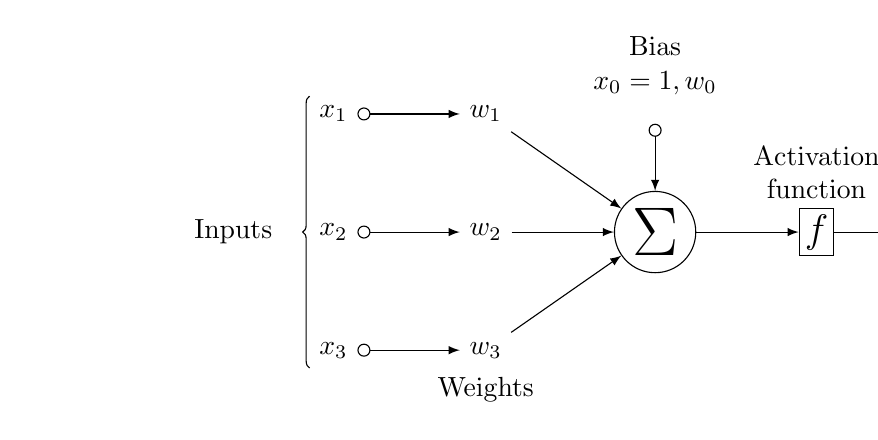
\begin{tikzpicture}[
  init/.style={
    draw,
    circle,
    inner sep=2pt,
    font=\Huge,
    join = by -latex
  },
  squa/.style={
    draw,
    inner sep=2pt,
    font=\Large,
    join = by -latex
  },
  start chain=2,node distance=13mm
  ]
  \node[on chain=2]
    (x2) {$x_2$};
  \node[on chain=2,join=by o-latex]
    {$w_2$};
  \node[on chain=2,init] (sigma)
    {$\displaystyle\Sigma$};
  \node[on chain=2,squa,label=above:{\parbox{2cm}{\centering Activation \\ function}}]
    {$f$};
  \node[on chain=2,label=above:Output,join=by -latex]
    {$y$};
  \begin{scope}[start chain=1]
  \node[on chain=1] at (0,1.5cm)
    (x1) {$x_1$};
  \node[on chain=1,join=by o-latex]
    (w1) {$w_1$};
  \end{scope}
  \begin{scope}[start chain=3]
  \node[on chain=3] at (0,-1.5cm)
    (x3) {$x_3$};
  \node[on chain=3,label=below:Weights,join=by o-latex]
    (w3) {$w_3$};
  \end{scope}
  \node[label=above:\parbox{2cm}{\centering Bias \\ $x_0=1, w_0$}] at (sigma|-w1) (b) {};

  \draw[-latex] (w1) -- (sigma);
  \draw[-latex] (w3) -- (sigma);
  \draw[o-latex] (b) -- (sigma);

  \draw[decorate,decoration={brace,mirror}] (x1.north west) -- node[left=10pt] {Inputs} (x3.south west);
  \end{tikzpicture}
\end{center}
\begin{figure}[b!]
  \centering
  \caption{Multi-layer fully connected network architecture}
  \label{fig:mlfc}
  \def\layersep{2.5cm}
  \begin{tikzpicture}[shorten >=1pt,->,draw=black!50, node distance=\layersep]
      \tikzstyle{every pin edge}=[<-,shorten <=1pt]
      \tikzstyle{neuron}=[circle,fill=black!25,minimum size=17pt,inner sep=0pt]
      \tikzstyle{input neuron}=[neuron, fill=green!50];
      \tikzstyle{output neuron}=[neuron, fill=red!50];
      \tikzstyle{hidden neuron}=[neuron, fill=blue!50];
      \tikzstyle{annot} = [text width=4em, text centered]

      % Draw the input layer nodes
      \foreach \name / \y in {1,...,4}
      % This is the same as writing \foreach \name / \y in {1/1,2/2,3/3,4/4}
          \node[input neuron, pin=left:Input \#\y] (I-\name) at (0,-\y) {};

      % Draw the hidden layer nodes
      \foreach \name / \y in {1,...,5}
          \path[yshift=0.5cm]
              node[hidden neuron] (H-\name) at (\layersep,-\y cm) {};

      % Draw the output layer node
      \node[output neuron,pin={[pin edge={->}]right:Output}, right of=H-3] (O) {};

      % Connect every node in the input layer with every node in the
      % hidden layer.
      \foreach \source in {1,...,4}
          \foreach \dest in {1,...,5}
              \path (I-\source) edge (H-\dest);

      % Connect every node in the hidden layer with the output layer
      \foreach \source in {1,...,5}
          \path (H-\source) edge (O);

      % Annotate the layers
      \node[annot,above of=H-1, node distance=1cm] (hl) {Hidden layer};
      \node[annot,left of=hl] {Input layer};
      \node[annot,right of=hl] {Output layer};
  \end{tikzpicture}
\end{figure}
\noindent As the reader can verify, the final decision about the magnitude of the signal is taken by the activation function. It is resposible to determine whether or not the input features are important enough to further contribute to the computation. The activation is a non-linear function, generally continuous and differentiable (except for very primitive formulations, like the perceptron \cite{rosenblatt1961principles}). These two properties are fundamental to build a multi-layered architecture. In fact, imagine to stack more than one layer of neurons as in Figure~\ref{fig:mlfc} where the output of the neurons are attached as inputs to the subsequent layer, then ideally, the larger the number of layers, the more ``learning power'' the network attains. Now, if the activation function was simply linear, regardless of how many layers are stacked, there would exist a single neuron that could approximate the same function, because the composition of linear functions is always just linear. Non-linearity solves this problem and enables deep architectures. But how do these artificial networks learn? Through trial and error, in a way that is arguably similar to the process of human learning. First, the inputs get propagated forward through the neurons until the output layer is reached and then the error is calculated with respect to the desired output value using a loss function. Intuitively, the loss represents the cost of the error, or a measure of the penalty the network will experience. Therefore, learning can be seen as an optimization problem that seeks to minimize the loss as objective function. The last building block needed for the network to improve its performance over time is the weight update through backpropagation (short for ``backward propagation of errors''). In fact, the weights of the neurons have a relationship with the error the network produces, thus, if the parameters make an adjustment in the right direction, the error decreases. The direction of the update is usually calculated by means of an optimization algorithm called gradient descent, that is based on the observation that a function decreases fastest if one goes in the direction of the negative gradient. Hence, given a learning rate $\gamma$ small enough, the loss $\mathcal{L}$, a weight vector $\theta$ and the following update:
\begin{equation}
  \theta_j \leftarrow \theta_j - \gamma\frac{\partial \mathcal{L}}{\partial \theta_j}
\end{equation}
then the loss is guaranteed to decrease. However, in the real case the learning rate is fixed so it is not mathematically certain that the performance will improve at each and every step, although it still works well in practice.\\
Neural networks are a very flexible tool that can be used for virtually every problem, yielding good performance. Neurons can be connected to each other in many ways, forming several architectures, in order to adapt them to different data types (images, sentences, etc.). Also, they can be used with good results in all the subfields of machine learning. The following two sections will explain how to build neural networks that are capable of processing images in both supervised and unsupervised settings.

\section{Semantic Segmentation}
Image segmentation is the partitioning of an image into several groups of pixels, also called segments, based on some criteria. The segments of an image are usually stored in a mask where each group is assigned a unique grayscale value or color to identify it. Image processing solutions to this problem, employing a wide range of criteria, have been deeply explored. Sometimes, it is posed as a graph partitioning problem \cite{shi2000normalized}, other times as a clustering task \cite{coleman1979image}. However, in general, these criteria do not make any attemps at understanding what the segments represent.\\
\begin{figure}[t]
    \centering
    \includegraphics[width=\textwidth]{./pictures/segmentation-masks}
    \caption{Examples of Semantic segmentation.}
    \label{fig:segmentation-masks}
\end{figure}\\
With the rise of Computer Vision the situtation changed completely. Instead of just applying some transformations to the image, Computer Vision aims to extract knowledge from the scene. Pixels are no longer seen as mere elements in a matrix, but rather as a means of conveying meaning. Performing image segmentation based on the understanding of the content is called semantic segmentation. Back in the 1990s, segmentation was carried out using probabilistic frameworks, like conditional random fields (CRFs) among the others. Their advantage is that they can model the relationship between pixels in order to be more accurate in the prediction of the label. Nowadays, CRFs are not really used anymore, except as post-processing step of neural network models. In fact, around 2006, a group of researchers brought together by the Canadian Institute for Advanced Research (CIFAR) showed that it is possible to train very deep artificial neural networks effectively \cite{hinton2006fast} and that they outperform any other algorithm on computer vision tasks \cite{hinton2006reducing}. It was the dawn of the Deep Learning era. The following years saw a rapid increase in the quantity of scientific articles using deep neural networks, tackling all sorts of problems that, until then, seemed unsolvable.
In the context of semantic segmentation this revolution led to the invention of fully convolutional networks (FCNs - Long et al.\cite{long2015fully}), a particular flavour of neural architecture that is able to produce pixel-level classification. Actually, the idea of using convolution-like operations to feed pixels into neurons first emerged in 1980 \cite{fukushima1980neocognitron} and ways of training them through backpropagation ware proposed around ten years later \cite{waibel1995phoneme}\cite{lecun1989backpropagation}.
Convolutional Neural Networks (CNNs) take advantage of the fact that the input consists of images and they constrain the architecture in a more sensible way. In particular, unlike a regular neural network, the layers (or filters) of a CNN have neurons arranged in 3 dimensions: width, height and depth (Figure~\ref{fig:conv-layer}). The neurons in a layer will only be connected to a small region of the layer that precedes them, instead of collecting the activations of all neurons in a fully connected manner \cite{cnn-stanford}. Using this trick has 2 advantages, first, it decreases the number of parameters to be learned by a large margin, second, it forces the model to learn hierarchically, concentrating on smaller regions of the image to capture local information, but then merging them together to deduce more high-level concepts. In practice, a CNN is able to encode the content of an image, automatically extracting features that are very effective at discriminating between classes, while at the same time preserving spacial information. This characteristic is fundamental because semantic segmentation faces an inherent tension between semantics and location: global information resolves ``what'' while local information resolves ``where''\cite{long2015fully}.
\begin{figure}[t]
    \centering
    \includegraphics[width=\textwidth]{./pictures/conv-layer}
    \caption{A visualization of a Convolutional Neural Network. In red the input image, in blue the convolutional layers, in green the output layer \cite{cnn-stanford}.}
    \label{fig:conv-layer}
\end{figure}
A FCN leverages the strenghts of this convolution-like operation to create an encoder-decoder architecture that is able to predict the location and the class of each object in the input. The encoder is a stack of convolutional, max pooling and batch normalization layers, where max pooling is a down-sampling operation that keeps the largest value, and batch normalization \cite{ioffe2015batch} handles the adjusting and scaling of the activations. The decoder is built similarly, but it up-samples the coarse feature maps into a full-resolution segmentation map using the transpose operation. The transpose convolutional filter does the opposite of a normal one, instead of performing a weighted sum of the inputs, it takes a single value, multiplies it by the weights of the filter and spreads the output values in the neighboring region of the next layer. Long et al. also added ``skip connections'' that take activations from the encoder and sum them up to the up-sampled features of the decoder. The information extracted from earlier layers in the network (prior to a down-sampling operation) should provide the necessary detail in order to reconstruct accurate shapes for segmentation boundaries.\\
\begin{figure}[t]
    \centering
    \includegraphics[width=\textwidth]{./pictures/u-net}
    \caption{U-Net architecture \cite{ronneberger2015u}.}
    \label{fig:unet}
\end{figure}\\
So, at training time, the network takes an image as input and propagates the values forward through the encoder and the decoder, until the output layer is reached. Subsequently, the error is calculated and the whole network is updated end-to-end using backpropagation. The loss function that leads the training should be carefully chosen, depending on the architecture and the specific problem that is being dealt with. However, in general, the good old cross entropy loss over each pixel can be used for segmentation:
\begin{equation}
\mathcal{L}(p, y) = -y\log(p)-(1-y)log(1-p)
\end{equation}
where $p$ is the predicted probability that a pixel belongs or not to the class and $y$ is the ground truth. This measure is a solid choice with regard to image segmentation, because it returns very stable gradients to the network and helps it converge smoothly. However, in some cases, cross entropy doesn't correlate well with human perception, especially when the distribution of the classes in the dataset is highly imbalaced. For this reason, other loss functions were introduced in the deep learning field. One of them is the Dice loss \cite{sudre2017generalised}, based on the Dice coefficient ($DC$) \cite{sorensen1948method}\cite{dice1945measures}, in formulas:
\begin{equation}
DC(X,Y) = \frac{2|X\cap Y|}{|X\cup Y|}
\end{equation}
where $X$ and $Y$ are respectively the set of pixels belonging to the predicted mask and the ground truth mask. Doing so, this coefficient quantifies the similarity (or overlap) between the real distribution of the classes and the one that was estimated by the network. \\
Among all the architectural proposals that followed the first FCN article \cite{long2015fully}, the one that most impacted the field was the U-Net \cite{ronneberger2015u}. Ronneberger et al. improve upon the vanilla version of the FCN primarily through improving the capacity of the decoder module of the network. More concretely, the strength of the U-Net consists in its symmetry, in other words the contracting path and the expanding path have roughly the same depth. In addition, the skip connections are revisited, in fact, in this architecture the features of the encoder are not summed to the ones of the decoder but rather concatenated. Thanks to these adjustments the U-Net produces much better results, being capable of distinguishing the details of objects from the background noise.\\
Over time, a wide range of more advanced atomic blocks got discovered and substituted to the original CNN blocks. This led to the pubblication of new versions of the U-Net. For example, in 2016, residual blocks \cite{he2016deep} were added to the architecture \cite{drozdzal2016importance} allowing faster convergence and deeper models to be trained. However, the simple but powerful ideas that laid the foundations for the U-Net still make it a very solid choice.

\section{Clustering}
Clustering is the process of identifying natural groupings or clusters within multidimensional data, based on some similarity measures \cite{omran2007overview}. Clusters differ from classes because they are not known a priori but they are rather extracted from the data. Clustering can be achieved by various algorithms that differ significantly in the way they model the data. Despite this, all of its various realizations belong to the unsupervised learning family. \\
The purpose of this section is not to compile a review of each and every clustering algorithm. For that, the reader should refer to the extensive literature on the topic that can be found in bibliography \cite{omran2007overview}\cite{jain1999data}. This section is more of a brief overview on the methods that will be used in our main algorithm and the more subtle tweaks that make clustering work well.\\
Broadly speaking, clustering can be divided into two subgroups: those that require a priori knowledge of the number of clusters and those that are able to infer it. This distincion is particularly important in the context of sunspot detection because humans are very good at deducing the number of sunspot groups intuitively. An example of an algorithm that needs to know the number of clusters before running is k-means. Became very popular because of its simplicity and efficiency, K-means belongs to the type of algorithms that model clusters as centroids. In fact, it initializes $k$ randomly selected centroids which are used as the beginning points for every cluster, and then performs iterative calculations to finding the least-squares assignment to centroids. The algorithm terminates when the centroids have stabilized or alternatively when the maximim number of iteration has been reached. K-means, as most clustering algorithms, is not guaranteed to return the globally best solution. To mitigate this issue, the procedure can be restarted randomly for a fixed number of times. Although k-means is not able to determine the number of clusters automatically some methods have been developed in order to fix this, like the silhouette method \cite{rousseeuw1987silhouettes} or the elbow method.
\begin{figure}[b!]
    \centering
    \includegraphics[width=\textwidth]{./pictures/dbscan}
    \caption{A visualization of DBSCAN running. Core points are highlighted in red, border points in yellow, outliers (noise) in blue}
    \label{fig:unet}
\end{figure}\\
\noindent In the panorama of clustering algorithms that do not require a prior estimate of the number of clusters, DBSCAN \cite{ester1996density} is one of the most famous. DBSCAN is based on a very different premise with respect to k-means. In fact it defines the clusters as dense connected regions in the data space. It takes 2 parameters as input:
\begin{itemize}
  \item \textbf{eps} ($\varepsilon$): the minimum distance between two points for them to be considered neighbors;
  \item \textbf{minPts}: the minimum number of points to form a dense region (core).
\end{itemize}
So, what happens at runtime is that a point is drawn from the dataset, DBSCAN forms an n-dimensional shape with radius $\varepsilon$ around that data point, and then counts how many data points (neighbors) fall within that shape. If the number of neighbors is at least \textit{minPts} then the selected point belongs to the core, otherwise it can be labeled as a border point or an outlier. Neighbors get expanded as well and the process continues until the density-connected cluster is completely found. Then, a new unvisited point is drawn and the same routine is repeated. The resulting clustering has the property that all the clusters have at least density $\varepsilon$. Therefore, DBSCAN works well under the assumption that the density of the clusters is homogeneous. Also, one of the advantages of using density is that it can be calculated using virtually any metric, while, by contrast, algorithms like k-means assume the points lay in an euclidean space. In any case in this thesis we will feed such algorithms with data representations learned to optimize their distribution in a euclidean space.

\section{Representation Learning}
Every day, when we read, hear a noise, see an object or, in other words, experience the world through senses our brains are flooded by information. One of the astonishing aspects of our intelligence is that we do not drown in this massive flow of data, but rather we are able to navigate through it. Much of the ability to draw the best from our perceptions is due to the way we represent information. In the human brain, sensory information is represented by neural activity. Recent studies proved that using the distribution of activation in the neural population generated by the sight of some object it is possible to reconstruct an image of the object itself \cite{shen2019deep}. This result suggests that the brain is constantly extracting salient features from perceptions.\\
Unsurprisingly, representation learning (also known as feature learning) is a fundamental step in almost any machine learning pipeline. Learning a representation means to find a model that maps a generic data point in a high-dimensional space to a set of latent variables in a low-dimensional space. Latent variables, as opposed to observable variables, are variables that are not directly observed but rather inferred. This feature transformation technique can be very useful because depending on how data is represented, different information can be uncovered. Nontheless, it is rarely used as a stand-alone procedure. To make the most out of it, representation learning should be coupled with other supervised or unsupervised techinques. In fact a good representation is one that makes a subsequent learning task easier \cite[Chapter~15]{goodfellow2016deep}.\\ % The choice of representation will usually depend on the choice of the subsequent learning task.
Many different approaches to representation learning are possible and some of them will be described here. The most straightforward way of discovering good descriptors for the data is through unsupervised learning. A statistical approach to representation learning is offered by the Principal Component Analysis (PCA) algorithm \cite{jolliffe2011principal}. PCA is a dimensionality reduction algorithm that uses an orthogonal transformation to convert a set of observations of possibly correlated variables into a set of linearly uncorrelated variables called principal components. The first principal component accounts for as much of the variability in the data as possible, and each succeeding component accounts for as much of the remaining variability as possible. Representations can be extracted from the principal components and used as inputs to other models. PCA is very popular and effective in some situations, but suffers many limitations due to the assumptions that is makes. One of the most criticized aspects is that it can only find linear correlations, but the relationships among data aren't always so simple. This assumption can be relaxed using models that are capable on non-linearity. Autoencoders are an example of this. They are particular types of neural networks that try to reconstruct their input. As in the case of image segmentation models, the architecture is composed by an encoder and a decoder, however, the interesting part here is not the output, but the bottleneck. The encoder is forced to produce a representation of the input that carries as much information as possible, in order for the decoder to be able to reconstruct the input. The features that are sampled at the bottleneck of the network can have several different properties, depending on the activation function and the loss that are used. Autoencoders can be used in combination with convolutional blocks as well, in order to extract features from images.\\
Clustering can also be considered an unsupervised feature learning algorithm. In fact, imagine to run, for instance, k-means on a dataset. The procedure will return $k$ centroids, where $k$ is the desired number of clusters. Features can be produced in several ways from the centroids. The simplest is to create a $k$-dimensional one-hot vector for each data point, where the $j$-th element of that vector is $1$ if the point belongs to the $j$-th cluster. It is also possible to use the distances to the clusters as features.\\
The situation changes when we have more information about the problem we want to solve. In fact we can train supervised learning models that look for the exact characteristics of the data that are most important to separate some predefined class. Imagine to have a dataset with 10 classes and to know the class associated to each record. Ideally, it is possible to train a model that is capable of taking two records as input and calculating their similarity. The model will be trained using the information about the classes as a supervision signal, for example the similarity can be defined to be $1$ when both inputs belong to the same class and $0$ otherwise. Once the model has converged, it can be used to predict the structure in unseeen data. In fact, there is plenty of clustering algorithms that are capable of taking a similarity matrix and find the clusters that optimize some measure. Hopefully then, each cluster will be trivially associated to the right class. This looks like a very far fetched approach in this case, because there are only 10 classes. With a low number of classes it is much easier to build a classifier that discerns them. But suppose to be working on Facebook's dataset of faces, where millions of people are catalogued. In this latter case, the classifier approach becomes unfeasible because it would have to decide among millions of classes, making complexity explode. On the other hand, for the similarity model this is not a problem, it just has more data to be trained on. In fact, pairwise similarity is still well defined and the large matrix that holds it doesn't have to be necessarily precomputed for the clustering phase. In practice, this model creates a different data representation by exploiting the relationships between the records. The new representation is indeed the similarity matrix.
\begin{figure}[b!]
    \centering
    \includegraphics[height=0.6\textheight]{./pictures/siamese}
    \caption{Siamese network architecture.}
    \label{fig:siamese}
\end{figure}\\
Several new studies elaborated on the concept that relative knowledge is, sometimes, a very powerful source to be drawn from. In the field of computer vision the solution to the problem of learning similarities in the data is called siamese network \cite{koch2015siamese}. The siamese network is a class of neural architectures that contain two or more identical subnetworks. Identical here means every aspect is shared, they have the same configuration, parameters and weights. In the case of two subnetworks, at training time each one takes one of the two input images and encodes it in a vector representation, also called embedding. The two outputs are then fed to a contrastive loss function \cite{hadsell2006dimensionality} defined as follows:
\begin{equation}
  \mathcal{CL}(D_{W_{12}}, y, m) = (y)\frac{1}{2}D_{W_{12}}^2 + (1-y)\frac{1}{2}max(0,m-D_{W_{12}})^2
\end{equation}
where $D_{W_{12}}$ is the distance between embedding $W_1$ and $W_2$, $y$ is the ground truth of the similarity and $m$ is the margin hyperparameter. The loss is called contrastive because it forces the model to learn how to embed images in such a way that neighbors are pulled together while, by contrast, non-neighbors are pushed apart. As the weights evolve during the training the updates are mirrored across both subnetworks. At testing time, all the images are embedded so that data becomes just a set of feature vectors. Any type of supervised or unsupervised learning algorithm can subsequently leverage the general representations generated by siamese networks. However, we will mainly focus on clustering methods that are able to group together all the realization of the same class in the test set. Representations can be learned in a way that optimizes clustering performance. It is sufficient to align the type of distance that is used by the contrastive loss and the clustering. So if, for instance, the distance $D_W$ in the loss is euclidean, then the clustering should be tuned accordingly to consider that the points lay in an euclidean space. Moreover, if the number of classes in the test set is not known a priori knowing the expected distance between the clusters could be very useful. Here the parameter $m$ comes into play. In fact, $m$ represents the margin after which the network won't push two dissimilar points further apart. It is therefore reasonable to assume that the expected distance between clusters will be roughly $m$.\\
Nowadays, the state of the art results for siamese networks are achieved using a slightly different version of the contrastive loss: the triplet loss. While the contrastive loss aims at relativey minimizing and maximizing the distance between similar (positive) and dissimilar (negative) examples separately, the triplet formulation does both things at the same time. Formally:
\begin{equation}
  \mathcal{TL}(D_{W_{ap}},D_{W_{an}}, m) = max(0,m+D_{W_{ap}}-D_{W_{an}})
\end{equation}
Where $D_{W_{ap}}$ is the distance between the anchor and and the positive example, $D_{W_{an}}$ between the anchor and the negative and $m$ is, again, the margin. The advantage with respect to the normal contrastive formulation is that, updating on both positive and negative cases concurrently you can manage to be less greedy, or alternatively to take into account more context. That said, sampling heuristic in such pairwise distance learning setting may be as crucial as choosing the right loss, as some studies state \cite{wu2017sampling}.

% \section{Complementary Methods}
% Deep neural networks are still very obscure and it is not straightforward to fully harness their power. Therefore, researchers came up with very ingenious stratagems to make them converge. In this section, some of the strategies that are currently being used to improve neural performance will be presented.
% \subsection{Optimizers}
% As already mentioned in this chapter, neural networks learn by an optimization algorithm called gradient descent. Yet, just using the vanilla version of it won't make the networks learn properly. Convergence can be slow for functions whose curvature varies chaotically depending on which direction the gradient points. Also, it causes the model to be very sensitive to the choice of the value of the learning rate, making the learning process unstable. Stochasting gradient descent (SGD) is an optimizer that builds upon gradient descent replacing the real gradient with a stochastic approximation. Instead of calculating the gradients for all of the training examples, it is sometimes more efficient to only use a random subset of these examples. By doing so, it increases the noise on the gradient but at the same time it acts like a regularizer to the gradient estimation, removing the bias of the training set. Regardless of stochasticity, a very simple way to accelerate optimizers is to introduce momentum. Rather than using only the gradient of the current step to guide the search, momentum also accumulates the gradient of the past steps to determine the direction to go. Adam \cite{kingma2014adam} combines adaptive momentum, SGD and other techniques to create the currently most used optimizer.
% \subsection{Multitask Learning}
% Convergence on very challenging tasks can be difficult and require a lot of computational resources. To accelerate the learni up Transfer Learning only aims at achieving high performance in the target task by transferring knowledge from the source task
% Rich Caruana defines multi-task learning as ``Multitask Learning is an approach to inductive transfer that improves generalization by using the domain information contained in the training signals of related tasks as an inductive bias. It does this by learning tasks in parallel while using a shared representation; what is learned for each task can help other tasks be learned better''\cite{caruana1997multitask}
% In the context of deep neural networks, multitask learning is achieved by architectures that have a bunch of shared layers and then task specific layers.
% Humans reuse knowledge from among different tasks to solve another task.
%
% shared features double check
% \subsection{CoordConv}

\chapter{Architettura del sistema}
\label{capitolo5}
\thispagestyle{empty}

% \chapter{Dataset}
\label{capitolo6}
\thispagestyle{empty}
\noindent The abundance of astronomical data provides great opportunities for machine learning. In fact, most of the data is free to use for anybody and labels are almost always available. Solar physics is no exception to that. Many public databases of solar events can be downloaded in textual form and then annotations can be reconstructed from them. However, the reconstruction is not trivial sometimes, since a good understanding of solar coordinate systems is required.\\
In this work 4 datasets have been merged together:
\begin{itemize}
  \item \textbf{Debrecen Photoheliographic Data (DPD) \cite{baranyi2016line}\cite{gyHori2016comparative}}: a catalogue of positions and areas of sunspots from 1974 until present times, compiled by using white-light full-disk observations taken at the Heliophysical Observatory of the Hungarian Academy of Sciences (Debrecen, Hungary) and its Gyula Observing Station as well as at other observatories;
  \item \textbf{Sunspot Index and Long-term Solar Observations (SILSO) Dataset \cite{clette2014revisiting}}: a time series of daily total sunspot number derived with the relative sunspot number formula \eqref{relssnum}, provided by the Royal Observatory of Belgium using a network of observers. This dataset will be used for validation and testing purposes only;
  \item \textbf{Virtual Solar Observatory (VSO) \cite{hill2009virtual}}: a tool for investigating the physics of the Sun, by searching and downloading existing databases for terrestrial and space-based observations;
  \item \textbf{US Air Force, Mount Wilson (USAF/MWL) Dataset}: a catalogue that provides a list of sunspot regions and their parameters, observed by the USAF solar observatories and the Mount Wilson observatory. In particular, it is famous for sunspot group classification data.
\end{itemize}
The last solar cycle was selected as a use case for the training and testing of the algorithm. Both ground and space telescope data were added up to form a quite large dataset. One full-disk observation was considered for each day, drawn and reconstructed from the DPD dataset. Space based data ranging from 2011 to 2014 was downloaded with a Python module called SunPy \cite{mumford2015sunpy} that connects to VSO's open APIs, while ground based data from 2011 to 2013 was obtained directly from DPD's FTP access. Due to availability problems, the ground observations for 2014 were missing from the database. Since the images came from different datasets some pre-processing was necessary to unify them. Ground based observations came in the form fits files with variable resolution (from 4096x4096 to 8192x8192), where limb darkening correction had already been applied but the disk was not centered in the the plate. So, first, the center, radius and axial tilt of the Sun were extracted from the header in order for the Sun to be aligned and cropped from the raw image. The coordinates of the sunspots were given in the DPD dataset in heliocentric-radial coordinates. From those, using simple trigonometry, it was easy to calculate the positions in pixel coordinates.
On the other hand, the preprocessing of space based observations needed a bit more work. For each day, sunpost instances were extracted from DPD, and SDO images were searched inside the VSO using date and time of the DPD observation. The temporally nearest image was selected and downloaded. Despite the fact that SDO observations are very frequent, the average delay between the image and the annotated mask was around half an hour on average. This time shift is pretty large, considering that the Sun rotates and the Earth moves on the orbit (SDO can be considered solidal to the Earth in this case). The misalignment was big enough to make it necessary to rotate the positions of the sunspots to create very accurate masks. Luckily, DPD also provides Carrington heliographic latitude and longitude for each sunspot. These coordinates can easily be transformed into the helioprojective system. At this point, the images were loaded as a SunPy Map, a class that contains many useful methods to interact with solar data. One of these functions allows to calculate where an helioprojective coordinate maps to, after a time delta, taking into account the differential solar rotation profile. This works well when the sunspots are big because the magnetic tubes that create them usually have a lot of ``inertia'', and therefore move pretty consistently with the rotation profile. Marginal misalignments still arise when sunspots are very small, because even a modest change in the magnetic perturbation causes erratic movements, making it difficult to predict their location. After these calculations, it was the turn of limb darkening correction. From the center of the disk, circles of increasing radius are created and the pixels that lay on the border of the circle are averaged, creating the limb darkening profile (blue points in Figure~\ref{fig:sldtk}). A polynomial function is fitted on these data points and then, for every pixel, the right correction is applied to straighten the profile.
\begin{figure}[t]
    \centering
    \includegraphics[width=\textwidth]{./pictures/SLDTk}
    \caption{Limb darkening intnsity profile created with SLDTk \cite{sldtk}.}
    \label{fig:sldtk}
\end{figure}\\
Once the coordinates of the sunspots are ready for both ground and space observations, the segmentation masks can be generated by a flooding procedure. For each sunspot a seed is initialized from its coordinates. From the seed, the procedure starts to explore the pixels around it in a breadth first fashion, so that for every iteration the pixels with lowest value are selected for expansion. By doing so, the algorithm floods the darkest areas of the image first, remaining trapped into the penumbra. Using the whole spot area provided by DPD, it is possible to calculte the exact number of pixels of each sunspot and therefore make the expansion stop exactly on the edge of the penumbra. All the pixels that have been selected at least once are then written on a black array that has the same shape of the original image, to create the segmentation mask. Actually, the final mask also contains information about the groups and their classes in order to train the second part of the algorithm. The annotations created by this procedure are consistently good in practice, as it can be appreciated from Figure~\ref{fig:annotated-sunspot}. The figure also shows how the precision of the mask increases with the size of sunspots. For instance, the contours of the small rightmost sunspots are not correctly captured in the mask, while the largest ones are almost perfectly represented.\\
\begin{figure}[t!]
    \centering
    \includegraphics[width=\textwidth]{./pictures/blanquish}
    \caption{Example of a sunspot group mask.}
    \label{fig:annotated-sunspot}
\end{figure}
Overall, data preparation was probably the hardest and most time consuming part of the work, but the results repay the effort. The final analysis on the dataset shows the following statistics:
\begin{itemize}
  \item 2555 images with 4K resolution;
  \item around 21000 sunspot group instances;
  \item around 190000 single sunspots;
\end{itemize}
However, in order to train the algorithm and be able to asses its performance, it is necessary to divide the dataset into three subsets:
\begin{enumerate}
  \item \textbf{training set}: the part of data the algorithm will learn from;
  \item \textbf{validation set}: the sample of data that is used to provide an unbiased evaluation of the model while tuning hyperparameters. In our case the validation set will be particularly useful to estimate the personal reduction coefficient ($k$);
  \item \textbf{test set}: the chunk of data that will be used to estimate the final performance of the model once it is completely trained.
\end{enumerate}
The dataset was split accordingly trying to minimize the dependencies among the subsets. The initial idea was to split the dataset randomly, sampling observations for each month. This would have enabled us to estimate more precisely the average monthly sunspot number in the testing phase, because the observations would have been homogeneously distributed. Unfortunately, this is not a good approach because it introduces strong dependencies in the data, since sunspots can last even more than ten days on the disk and therefore the same sunspot could have appeared in both training and test data. A simple strategy is to divide the dataset while reducing regularities is to sample observations consecutively for the validation and test sets. So for each month the data was partitioned as follows:
\begin{itemize}
  \item days from the 1\textsuperscript{st} to the 19\textsuperscript{th} were assigned to the training set;
  \item days from the 20\textsuperscript{th} to the 24\textsuperscript{th} were assigned to the validation set;
  \item days from the 25\textsuperscript{th} to the last one of the month were assigned to the test set;
\end{itemize}
This data split design doesn't completely solve the dependency problem. In fact, though harder, it is still possible that the same sunspot appears repeated among the three sets. However, the longer the sunspot survives on the disk the more deformation it undergoes, strongly mitigating the dependency issue. Also, this partitioning strategy is a good trade-off because it still enables us to make monthly activity charts, averaging the results over the test set.
\clearpage

% \chapter{The Model}
\label{capitolo7}
\section{Training}
\subsection{Full-Disk Image Segmentation}
\noindent We argued that the problem of estimating the activity of the Sun ultimately reduces to the calculation of the relative sunspot number. A fundamental step for this calculation is finding the number of single sunspots in a full-disk image of the Sun. Semantic segmentation was selected as a tool to identify the areas of the disk that contain a sunspot, intended as all the pixels that fall inside the border of the penumbra, as opposed to the areas where the Sun is quiet.
\bigbreak
\noindent In practice, we need a model that is able to take an image as input and return a binary segmentation mask, where all and only the pixels belonging to some sunspot have a predicted label equal to 1. Unfortunately, this is not sufficient to be able to count them. In fact, depending on the class of the group, two or more sunspots can be surrounded by the same penumbra. Therefore it becomes necessary to separate umbras from penumbras as well. This can be achieved with a mix of classification and clustering techinques applied on the results of the segmentation model. This further refinement of the counting routine was not performed at training time and therefore is addressed in Chapter~\ref{capitolo6}.
\bigbreak
\noindent Starting with the semantic segmentation step, the first component of the program that counts the sunspots is a deep neural network for image segmentation. Specifically, the architecture that was chosen in this case is the U-Net. Minor changes to its internal structure were made to adapt it to the particular porblem, but the overall functioning  is the same as explained in Section \ref{autoannotation}. With respect to the original configuration, the network was made considerably more efficient by decreasing the number of convolutional filters in each layer, without though decreasing performance.
\bigbreak
\noindent At training time input images of the disk are divided into an array of overlapping patches and for each one of them the number of non-zero pixels in the respective patch of the ground truth mask is calculated. The number of non-zero pixels is considered as a measure of the salience, or equivalently an indication of how much the network can learn from such patch. At the same time, the number of patches to be extracted ($n_p$) is determined using a simple heuristic that takes into account the number of groups that are present in the image. Then, $n_p$ patches are sampled from the array with probability proportional to the salience of the patch. This procedures enables the network to draw the best from each training episode, since the images are very large, while the sunspots are small and concentrated in the equatorial band of the disk.
\bigbreak
\noindent Now that the training examples have been identified, it is the time of feeding them into the U-Net. The patches are organized in a batch and forwarded into the network. When the computation has finished, the output layer returns the predicted mask for each input example. These masks are compared to the real masks and the error is calculated using cross entropy loss. Subsequently, the error is backpropagated through the network so that the optimization of the parameters can be performed. The optimizer that was used on this network is called stochastic gradient descent (SGD) and it works by replacing the real gradient with a stochastic approximation. Instead of calculating the gradients for all of the training examples, it is sometimes more efficient to only use a random subset of these examples. By doing so, it increases the noise on the gradient, but at the same time it acts like a regularizer to the gradient estimation, removing the bias of the training set. Also, momentum was used in combination with SGD. With momentum the optimizer accumulates the gradient of the past steps to determine the direction to go, rather than using only the current step to guide the search. The combination of these two strategies helped the network converge and become very good at telling sunspots apart from quiet disk areas. Examples results on the training and validation sets are shown in Figure~\ref{fig:pred-vs-ground}, while the reader can take a look at a predicted mask and compare it to the ground truth mask in Figure~\ref{fig:cross-entropy-loss}.
\bigbreak
\noindent A detailed look at the results made it clear that the model has a quite good and qualitative understanding of the concept of sunspot, attaining good performance, regardless of the fact that the sunspot is located on the center of the disk or on the limb. Moreover, the U-Net learns to overcome the limitations of the ground truth due to weak supervision. When sunspots are very small it looks like the network does a better job than the rotation routine at localizing them. This behaviour, together with the fact that the patches are sampled differently on each epoch, generates the high variance of the results (Figure~\ref{fig:cross-entropy-loss}). A summary of the whole training phase can be examined in Figure~\ref{fig:workflow}.
\clearpage
\begin{figure}[t!]
    \centering
    \captionsetup{justification=centering}
    \includegraphics[width=\textwidth]{./pictures/pred-vs-ground}
    \caption{Comparison between the predicted mask (green) and the ground truth (red).}
    \label{fig:pred-vs-ground}
\end{figure}
\begin{figure}[t!]
    \centering
    \captionsetup{justification=centering}
    \includegraphics[width=\textwidth]{./pictures/cross-entropy-loss}
    \caption{U-Net convergence curve on the training set.}
    \label{fig:cross-entropy-loss}
\end{figure}
\clearpage
\begin{figure}[h]
    \centering
    \captionsetup{justification=centering}
    \includegraphics[width=\textwidth]{./pictures/workflow}
    \caption{Summary of the training of the segmentation phase}
    \label{fig:workflow}
\end{figure}
\clearpage
\subsection{Sunspot Representations and Classification}
Probably, the part of the sunspot index estimation that requires most expert knowledge is the determination of the number of groups. The setting of the problem is mainly unsupervised, because groups change every day and there is no predefined category that generalizes from one day to another.
\bigbreak
\noindent  Clustering seems a very natural approach for this problem. It is indeed, but it is also desirable to leverage the datasets of annotated sunspot groups that are available online to make the algorithm mimic the way humans cluster sunspots. A sensible form of blending together a supervised model with clustering is by using the labels to create good representations of the data. Specifically, we want to take the image of a sunspot and remap it to a feature vector that optimizes the result of the subsequent step. This can be achieved by training a siamese network that embeds sunspots in a way that separates them according to the configuration of the groups. To guide the neural network in the search of the optimal features to extract, a contrastive loss is applied. After the mapping is performed, clustering can be employed to find the number of groups.
\bigbreak
\noindent At each training episode a ground truth mask that also contains the instances of the clusters is loaded from the dataset. From every group that is present on the disk, an anchor sunspot is randomly chosen. If the sunspot is not alone in the group, a positive example is selected from the same group. Similarly, a negative example is chosen from the other clusters if they exist. A square patch is centered and cropped from the full-disk image for each example that has been sampled. Now, the visual appearence of the sunspot is certainly an important feature, but its position and its total area are crucial as well. So, how can we give this features as inputs to the siamese network? Recent studies have shown that coordinates can be given as input to convolutional neural networks to improve their performance \cite{liu2018intriguing}. Thus, the centroids of each sunspot in heliographic coordinates are appended as a channel to the input tensor (the coordinate value is repeated on the whole channel). The same is done with the value of the area, after having it normalized by the total area of the disk. The final input tensor to the convolutional layers has therefore 4 channels (as it can be seen in Figure~\ref{fig:siamese-workflow}) holding respectively:
\begin{itemize}
  \item 1 channel for the patch of the image that contains the sunspot;
  \item 2 channels for the heliographic latitude and longitude;
  \item 1 channel for the normalized area of the sunspot.
\end{itemize}
After the tensor is propagated, the convolutaional layers produce an intermediate representation that, in turn, passes through two fully connected layers, generating a 5-dimesional embedding as output. This procedure gets repeated for all the selected sunspots and for each one of them the loss tries to pull the positive matches together (low Euclidean distance) while pushing the negative ones apart (high Euclidean distance).
\bigbreak
\noindent At the same time, the convolutional layers are repurposed for classification. The intermediate representation generated by the convolutional layers is also fed to a second, almost identical fully connected block that deals with classification. In this case, the desired output is the modified Z\"{u}rich class (Z component of the McIntosh classification). Identifying the type of sunspot that is being processed is important because the presence of penumbra surrounding the umbra can be derived directly from the class. As always, the classification error (calculated with the standard cross entropy loss) is backpropagated through the layers. Note that the fully connected layers only receive the gradients coming from their own output while the shared convolutional layers accumulate the gradients coming from both the contrastive loss and the cross entropy loss.
\bigbreak
\noindent This type of learning paradigm, where the network solves two or more problems at the same time, is called multitask learning \cite{caruana1997multitask}. It is based on the idea that what is learned for each task can help other tasks be learned better. This is indeed the case for sunspot clustering. In fact, even humans use group classification as an aid in the process of grouping them together.
\bigbreak
\noindent The process of training this ``two-headed'' architecture was very hard, due to the fact that the way positive and negative examples are selected makes a very big impact on the final result. Nonetheless, finally, it was possible to make the network learn both tasks with very good performance. The training curves can be examined in Figure~\ref{fig:siamese-training}.
\begin{figure}[hb!]
  \centering
  \captionsetup{justification=centering}
  \includegraphics[width=\textwidth]{./pictures/siamese-workflow}
  \caption{Summary of the training of the siamese network}
  \label{fig:siamese-workflow}
\end{figure}
\begin{figure}[h!]
    \centering
    \captionsetup{justification=centering}
    \begin{subfigure}[t]{\textwidth}
        \includegraphics[width=\textwidth]{./pictures/contrastive-loss}
    \end{subfigure}\vspace{3mm}
    \begin{subfigure}[t]{\textwidth}
        \includegraphics[width=\textwidth]{./pictures/classification-loss}
    \end{subfigure}
    \caption{Multitask siamese network convergence curve. Note that the implementation of the contrastive loss that has been used constrains the minimum possible value to be 0.5}
    \label{fig:siamese-training}
\end{figure}
\clearpage
\section{Automatic Annotation Procedure}
\label{autoannotation}
After both components of the model have been trained, it is time to join them in order to make predictions on unseen data. However, just stacking the U-Net and the siamese network together is not sufficient and other subcomponents are added. In this section we aim at describing in detail all the steps that are necessary to compose a successful annotation algorithm.
\bigbreak
\noindent Contrary to the training phase, the loading routine is now very simple, since it just needs to fetch the image that is annotated and no mask is needed (it is produced automatically). So, the prediction routine starts loading the image and dividing it into patches, while the parameters of the two neural networks get restored from selected checkpoints. One by one, the patches get sent into the U-Net that takes care of the first segmentation stage. As soon as the whole image has been evaluated, the mask gets reconstructed from the patches. Note that, since the U-Net outputs probabilities, every pixel has a continuous value (between 0 and 1) that needs to be rounded with a threshold in order to obtain a mask where the background has value 0 and the sunspot areas have value 1.
\bigbreak
\noindent At this point, we know with good confindence that the parts of the image that have been highlighted from the U-Net contain one or more sunspots each. To use this information for the subsequent steps we first need to convert it to a more usable form. The mask is, scanned looking for connected componets of pixels with value 1. At the same time, statistics are extracted for every component and the data is organized in an array. It is precisely from this information that the inputs for the siamese network are created. In fact, similarly to what was done during training time, the input channels are built using respectively a centered patch, the coordinates of the centroid and the area of the connected components. Coordinates are now in pixel space so they need to be translated to the heliographic system via trigonometry. When this is done, the data is forwarded through the convolutional layers of the siamese network and then the two fully connected heads are evaluated in parallel. The network outputs both the embeddings and the classes of each connected component.
\bigbreak
\noindent From this moment on, the computaton splits in two branches, one that seeks to refine the quality of the segmentation to yield the number of single sunspots, the other that finds the number of groups and assigns each sunspot to one of them.
\begin{figure}[ht!]
  \centering
  \captionsetup{justification=centering}
  \includegraphics[width=\textwidth]{./pictures/histograms}
  \caption{Comparison between histograms of the same patch, with or without the mask}
  \label{fig:histograms}
\end{figure}
Refining the quality of the segmentation mask means, in this context, to be able to separate the umbra from the penumbra of each connected component of pixels generated by the U-Net. This operation is important because more than one umbrae can be surrounded by the same penumbrae, affecting the sunspot count. First, it is necessary to understand if the sunspot exhibits or not the penumbra. This is easy considered that we can leverage the classification produced by the siamese network together with some simple heuristic concerning the area of the sunspot.
\bigbreak
\noindent Classes \textbf{A} and \textbf{B} imply that the sunspots of the group do not have penumbra while classes \textbf{C} to \textbf{H} all expect penumbra. Small sunspots that usually locate at the periphery of groups are directly discarded with some threshold on the value of the area since we assume that they are very unlikely to carry more than one umbra. This knowledge enables us to segment the connected component using its histogram. In fact, since the division between umbra and penumbra creates a strong intensity discontinuity, the cut-off value is evident in the histogram if the mask of the whole sunspot is known a priori. Referring to Figure~\ref{fig:histograms} as an aid to visualization, the two peaks that can be seen around pixel value 30 and 130 are respectively the umbra and the penumbra. Given this knowledge of the problem we can proceed with two approaches, either fitting two gaussians and assigning each pixel to the most likely one, or simply perforoming clustering in one dimension fixing the number of clusters to the value 2. Both solutions were explored during the development of this work but in the end clustering was selected because, despite being simpler, it yields the same performance.
\bigbreak
\noindent At the end, the refinement of the segmentation step reduces to running k-means on the mask generated by the U-Net. The two clusters of pixels are then used to create a new mask that only highlights umbras, and the number of connected components is recalculated from it.
\bigbreak
\noindent The second branch of the procedure finds the number of groups and assigns each sunspot (connected component of pixels) to one of them, using the embeddings created by the siamese network. Those embeddings are created to optimize the positions of the connected components in a 5-dimensional Euclidean space. As already treated in the previous section, the optimization operated by the siamese network lies in the fact that sunspots belonging to the same group should be close together in the Euclidean space. This is, once again, a great opportunity to unleash the potential of clustering algorithms. However, the main difficulty here is that the number of clusters is not known beforehand, because it is indeed the value that we want to calculate.
\bigbreak
\noindent DBSCAN seems like a very good match for this problem. In fact, it just needs two parameters: $eps$ ($\varepsilon$) which can be estimated statistically on the validation set (see next section) and $minPts$ which is trivially set to 0 (otherwise groups composed by a lone sunspot would be interpreted as outliers). Given the parameters and the embeddings as inputs, DBSCAN reliably returns the number of clusters that is useful for later computations.
\bigbreak
\noindent Now that the image has been annotated and the number of groups and single sunspots is known it is sufficient to find the personal reduction coefficient to be able to calculate the final value of the relative sunspot number. The estimation of the personal reduction coefficient and the $eps$ ($\varepsilon$) parameter for DBSCAN are addressed in the next section.

\section{Parameter Estimation}
The validation set provides an exceptional opportunity for the estimation of parameters. In fact, many instances of the algorithm can be run using the data that was held out from the training set, so the variation in performance can be assessed. Various combinations of parameters can be evaluated and the best model can be then used to draw the final results on the test set.
Among the others, two parameters have been studied in detail in this work:
\begin{itemize}
  \item the $eps$ ($\varepsilon$) parameter for DBSCAN that represent the minimum distance between two points for them to be considered neighbors;
  \item the personal reduction coefficient ($K$) of the algorithm, compared to the international sunspot number provided by SILSO.
\end{itemize}
These two parameters are not independent from each other and therefore they were tested in two consecutive phases, both on the whole validation set.
\bigbreak
\noindent The first one that needed to be assessed was the value of $eps$. The number of clusters detected from DBSCAN dramatically depends on this parameter, so optimizing it is vital to improve the final performance. Although the variable that drives the performance is the number of clusters, we didn't use it as the measure to optimize $eps$ because it is not informative enough. Instead, the Adjusted Random Index (ARI), a performance index that takes into account the configuration of points inside the clusters and compares it to the ground truth was used. ARI is defined as:
\begin{equation}
ARI = \frac{RI-\mathbb{E}[RI]}{max(RI)-\mathbb{E}[RI]}
\end{equation}
where $RI$ (Rand Index) is the number of pairs of objects that are either in the same group or in different groups in both partitions divided by the total number of pairs of objects. The ARI performs a correction with respect to the Rand index in order to account for the variability of the expected value of two random partitions. Thus, the ARI has a value close to 0 for random labeling independently of the number of clusters and exactly 1 when the clusterings are identical.
\bigbreak
\noindent We tested the algorithm 50 times on the whole validation set, each time with a different value for the $eps$ parameter. The results are shown in Figure~\ref{fig:eps-ari}. After the estimation of the curve it is possible to take the value that maximizes the performance index and use it as input for the subsequent tests.
\bigbreak
\noindent After $eps$, we proceded to estimate the value of the reduction coefficient $K$ using a similar procedure. This time, instead of maximizing some performance index, the task is to minimize the deviation of our calculation of the sunspot number from the international sunspot index provided by SILSO. This can be achieved using the root-mean-square (RMS) error between the two calculations over the whole validation set. The procedure was repeated 100 times with values of $K$ ranging from 0 to 2 (Figure~\ref{fig:k-rms}). The optimal minimal error is attained when the $K$ coefficient takes the value 0.58. Such a low value for $K$ is explained by the fact that the images that have been used by our algorithm come from the best observatories in the world. Depending on the optics of the telescope, the amount of detail that can be resolved changes. So, in general, the better the optics, the more sunspots it captures. For this reason, the estimation our algorithm provides is high, and therefore it should be multiplied by a low value to align to the international sunspot number.\clearpage
\begin{figure}[ht!]
  \centering
  \captionsetup{justification=centering}
  \includegraphics[width=\textwidth]{./pictures/eps-ari-copy}
  \caption{ARI value for varying $eps$ values}
  \label{fig:eps-ari}
\end{figure}
\begin{figure}[h!]
  \centering
  \captionsetup{justification=centering}
  \includegraphics[width=\textwidth]{./pictures/k-rms-copy}
  \caption{RMS error value for varying $K$ value}
  \label{fig:k-rms}
\end{figure}


\cleardoublepage
% ---- Bibliography ----
\pagestyle{plain}
\addcontentsline{toc}{chapter}{Bibliography}
\bibliographystyle{unsrt}
\bibliography{bibliography}

%\nocite{*}

\appendix

\pagestyle{fancy}
\fancyfoot{}
\renewcommand{\chaptermark}[1]{\markboth{\appendixname\ \thechapter.\ #1}{}}
\renewcommand{\sectionmark}[1]{\markright{\thesection.\ #1}}
\fancyhead[LE,RO]{\bfseries\thepage}

\fancyhead[RE]{\bfseries\leftmark}
\fancyhead[LO]{\bfseries\rightmark}
\renewcommand{\headrulewidth}{0.3pt}

% \chapter{Glossary}
\label{appendiceA}
\thispagestyle{empty}

The definitions in this glossary are taken from NOAA's space weather glossary \cite{NOAAglossary}.\\


\newenvironment{myindentpar}[1]%
{\begin{list}{}%
        {\setlength{\leftmargin}{#1}}%
        \item[]%
}
{\end{list}}


\textbf{Active Region:}
\begin{myindentpar}{1cm}
  A localized, transient volume of the solar atmosphere in which plages, sunspots, faculae, flares, etc. may be observed.
\end{myindentpar}

\textbf{Aurora:}
\begin{myindentpar}{1cm}
A faint visual (optical) phenomenon on the Earth associated with geomagnetic activity, which occurs mainly in the high-latitude night sky. Typical auroras are 100 to 250 km above the ground. The Aurora Borealis occurs in the northern hemisphere and the Aurora Australis occurs in the southern hemisphere.
\end{myindentpar}

\textbf{Corona:}
\begin{myindentpar}{1cm}
  The outermost layer of the solar atmosphere, characterized by low densities and extraordinarily high temperatures that extends to several solar radii. The heating of the corona is still a mystery. The shape of the corona is different at solar maximum and at solar minimum.
\end{myindentpar}

\textbf{Coronal Hole:}
\begin{myindentpar}{1cm}
  An extended region of the corona, exceptionally low in density (large open "gaps"), and associated with photospheric regions. Coronal holes are closely associated with those regions on the Sun that have an "open" magnetic geometry, that is, the magnetic field lines associated with them extend far outward into interplanetary space, rather than looping back to the photosphere. Ionized material can flow easily along such a path, and this in turn aids the mechanism that causes high speed solar wind streams to develop.
\end{myindentpar}

\textbf{Coronal Mass Ejection:}
\begin{myindentpar}{1cm}
  An observable change in coronal structure that occurs on a time scale between a few minutes and several hours, and involves the appearance of a new discrete, bright, white light feature in the coronagraph field of view, that displays a predominantly outward motion. The solar corona material is massive in size (they can occupy up to a quarter of the solar limb), and frequently accompanied by the remnants of an eruptive prominence, and less often by a strong solar flare. The leading edges of fast-moving CMEs drive giant shock waves before them through the solar wind at speeds up to 1200 km per second. Some astronomers believe that CMEs are the crucial link between a solar disturbance its propagation through the heliosphere, and the effects on the Earth.
\end{myindentpar}

\textbf{Differential Rotation:}
\begin{myindentpar}{1cm}
  The change in solar rotation rate with latitude. Low latitudes rotate at a faster angular rate (approx. 14 degrees per day) than do high latitudes (approx. 12 degrees per day). For example, the equatorial rotation period is 27.7 days compared to 28.6 days at latitude 40 degrees.
\end{myindentpar}

\textbf{Disk:}
\begin{myindentpar}{1cm}
  The visible surface of the Sun (or any heavenly body) projected against the sky.
\end{myindentpar}

\textbf{Eruptive:}
\begin{myindentpar}{1cm}
  Solar activity levels with at least one radio event and several chromospheric events per day.
\end{myindentpar}

\textbf{Facula:}
\begin{myindentpar}{1cm}
  A bright cloud-like feature located a few hundred km above the photosphere near sunspot groups, seen in white light. Facula are seldom visible except near the solar limb, although they occur all across the Sun. Facula are clouds of emission that occur where a strong magnetic field creates extra heat (about 300 degrees K above surrounding areas).
\end{myindentpar}

\textbf{Filament:}
\begin{myindentpar}{1cm}
  A mass of gas suspended over the photosphere by magnetic fields and seen as dark lines threaded over the solar disk. A filament on the limb of the Sun seen in emission against the dark sky is called a prominence.
\end{myindentpar}

\textbf{Flux:}
\begin{myindentpar}{1cm}
  The rate of flow of a physical quantity through a reference surface.
\end{myindentpar}

\textbf{Geomagnetic Field:}
\begin{myindentpar}{1cm}
  The magnetic field observed in and around the Earth. The intensity of the magnetic field at the Earth's surface is approximately 0.32 gauss at the equator and 0.62 gauss at the north pole.
\end{myindentpar}

\textbf{H-alpha:}
\begin{myindentpar}{1cm}
  This absorption line of neutral hydrogen falls in the red part of the visible spectrum and is convenient for solar observations. The H-alpha line is universally used for observations of solar flares and prominences.
\end{myindentpar}

\textbf{Helioseismology:}
\begin{myindentpar}{1cm}
  A method for studing the Sun by utilizing waves that propagate throughout the star to measure its invisible internal structure and dynamics.
\end{myindentpar}

\textbf{Limb:}
\begin{myindentpar}{1cm}
  The edge of the solar disk.
\end{myindentpar}

\textbf{Magnetogram:}
\begin{myindentpar}{1cm}
  Solar magnetograms are a graphic representation of solar magnetic field strengths and polarity.
\end{myindentpar}

\textbf{Penumbra:}
\begin{myindentpar}{1cm}
  The sunspot area that may surround the darker umbra or umbrae. It consists of linear bright and dark elements radial from the sunspot umbra.
\end{myindentpar}

\textbf{Plasma:}
\begin{myindentpar}{1cm}
  Any ionized gas, that is, any gas containing ions and electrons.
\end{myindentpar}

\textbf{Prominence:}
\begin{myindentpar}{1cm}
  A term identifying cloud-like features in the solar atmosphere. The features appear as bright structures in the corona above the solar limb and as dark filaments when seen projected against the solar disk.
\end{myindentpar}

\textbf{Quiet:}
\begin{myindentpar}{1cm}
  Solar activity levels with less than one chromospheric event per day.
\end{myindentpar}

\textbf{Solar Cycle:}
\begin{myindentpar}{1cm}
  The approximately 11-year quasi-periodic variation in frequency or number of solar active events.
\end{myindentpar}

\textbf{Solar Maximum:}
\begin{myindentpar}{1cm}
  The month(s) during the solar cycle when the 12-month mean of monthly average sunspot numbers reaches a maximum.
\end{myindentpar}

\textbf{Solar Minimum:}
\begin{myindentpar}{1cm}
  The month(s) during the solar cycle when the 12-month mean of monthly average sunspot numbers reaches a minimum.
\end{myindentpar}

\textbf{Umbra:}
\begin{myindentpar}{1cm}
  The dark core or cores (umbrae) in a sunspot with penumbra, or a sunspot lacking penumbra.
\end{myindentpar}

\textbf{White-Light:}
\begin{myindentpar}{1cm}
  Sunlight integrated over the visible portion of the spectrum (4000 - 7000 angstroms) so that all colors are blended to appear white to the eye.
\end{myindentpar}

% \chapter{McIntosh Classification Example Images}
\label{appendiceB}
\thispagestyle{empty}
Figure \ref{fig:mcintosh} shows example images taken from SDO for each McIntosh class.
\begin{figure}[h!]
    \centering
    \captionsetup{justification=centering}
    \includegraphics[width=0.93\textwidth]{./pictures/mcintosh-classification}
    \caption{Example images taken from SDO for each McIntosh class}
    \label{fig:mcintosh}
\end{figure}

% \chapter{Helios Processing Pipeline}
\label{appendiceC}
\thispagestyle{empty}
This appendix describes the first part of the work that was done at the Helios observatory of the European Space Agency. The observatory belongs to the CESAR (Cooperation through Education in Science and Astronomy Research) initiative, whose objective is to provide students from european secondary schools and universities with hands-on experience in Astronomy research in general and in Radio Astronomy and Optical Astronomy in particular. Helios was installed at ESAC (European Space Astronomy Centre) in 2012 and includes two telescopes (Figure wanama):
\begin{itemize}
  \item Coronado Solarmax II 90, H-alpha, double stack, with specifications:
  \begin{itemize}
    \item Aperture: 90mm
    \item Focal Length: 800mm
    \item Bandwidth: \textless0.5 \AA
  \end{itemize}
  \item Bresser AR-102, visible (white-light), with specifications:
  \begin{itemize}
    \item Aperture: 102mm
    \item Focal Length: 1000mm
    \item Solar Filter: BAADER AstroSolar Safety Filter
  \end{itemize}
\end{itemize}
\bigbreak
The two telescopes are mounted on the same robotic arm (Figure wanama) and are very different from each other. The main difference is in the type of filter they have on board. On the one hand, the filter that comes with the Coronado Solarmax isolates the H-alpha band, a deep-red visible spectral line. H-alpha is particularly useful in solar astronomy because it enables the observation of the atmosphere of the Sun. On the other hand, the filters that are used for white-light observation do not reduce the portion of the specturm that enters the scope, but rather decrease the intesity of the radiation. Therefore each pixel of the sensor, attached at the bottom of the scope, receives the whole visible spectrum and integrates it to obtain the total intensity.
\bigbreak
\begin{figure}[t!]
    \centering
    \captionsetup{justification=centering}
    \includegraphics[height=0.4\textheight]{./pictures/solar-telescopes}
    \caption{A picture of the two telescopes}
    \label{fig:pred-vs-ground}
\end{figure}
Given these differences, dedicated processing techniques are used for each telescope. Nonetheless, the preliminary steps of the two pipelines are shared, although with different parameters, and they are therefore presented together. In fact, we can logically divide the pipelines in two phases (which are treated in the next sections):
\begin{itemize}
  \item \textbf{Preliminary adjustments}, performed for both telescopes with different parameters;
  \item \textbf{Feature enhancement}, dedicated for each telescope.
\end{itemize}

\section{Preliminary Adjustments}
The first phase of the processing starts with a set of quality control checks. For each image we need to make sure that they are not corrupted or completely black, since files could be damaged during the transfer from the observatory to the servers that are allocated for the processing. Then, a second check, called cloud control, is performed to retain only the images where the Sun is perfectly visible, and discard the cloudy ones.
\bigbreak
Once it is certain that the images are up to standard, the pipeline proceeds to perform some corrections that are necessary to remove the artifacts introduced by the sensor. In fact, even the best sensors suffer from variations in the pixel sensitivity of the detector and distortions in the optical path. Luckily, is possible to account for these errors unsing two techniques that are really popular in digital photograpy: \textbf{dark-frame subtraction} and \textbf{flat-field correction}. The former tries to minimize the noise due to defective pixels and dark currents, while the latter adjusts for the relative sensitivity of pixels. The dark-frame is created by taking long exposure images in con complete darkness, or, in this case, when the lid of the telescope is on. The flat-field, instead, is generated attaching an omogeneous light source over the instrument, to measure how much each pixel reacts to it. Thus, two calibration images are used to adjust the images with the following formula:
\begin{equation}
C = \frac{(R - D)}{(F - D)}
\end{equation}
where $C$ is the corrected image, $R$ is the raw image, and $F$ and $D$ are the flat-field and the dark-frame respectively.
\bigbreak
The third subphase of the preliminary adjustments phase deals with image centering and axial tilt correction. Although, as explained in Appendix D, the telescope itself and the master control program already account for the tracking of the Sun, the limited accuracy of mechanical arms makes it necessary to use image processing techniques to align and center the solar disk to the frame. Moreover, in this case, centering the image is made easier by the fact that the shape of the object we are looking for is known and its size can be calculated with simple geometry. In fact, first, the sun can be considered a sphere, since its oblateness is neglectable; and second, the size of the appearent radius can be determined from the Sun-Earth distance. For the latter calculation it is sufficent to know the radius at one point of the orbit (we used the perihelion), and remember that the appearent size of an object is proportional to its distance. Therefore the radius can be calculated as:
\begin{equation}
  R = R_p\frac{d}{d_p}
\end{equation}
where $R$ is the desired radius in pixels at distance $d$, and $R_p$ and $d_p$ are respectively the radius and the distance at perihelion.
\bigbreak
Knowing the appearent radius for each day, it is possible to build a dynamic template of the disk, and template matching can be applied to find the center of the Sun in pixel coordinates. Also, the radius can be used to determine the size of the patch to be cropped in order to obtain an image in which the Sun is centered. The perfect alignment is achieved by rotating the resulting image by an angle that is equal to the axial tilt.

\section{Feature Enhancement}
\subsection{White-light}















- mean and std dev
- gradient sharpening
- limb darkening correction




\subsection{H-alpha}

- off limb emission enhancement
- kernel sharpening

% Given these differences, dedicated processing techniques are used to extract specific features from the raw images of each telescope.  In fact, the two pipelines
























% end

% \chapter{Il manuale utente}
\label{appendiceD}
\thispagestyle{empty}

% \chapter{Esempio di impiego}
\label{appendiceE}
\thispagestyle{empty}

% \chapter{Datasheet}
\label{appendiceF}
\thispagestyle{empty}


\end{document}
